
\section{Introductions}

Firstly, I want to thank for a chance to be a candidate for the Data team and an exciting challenge. I am on my way to finish my study and complete my final thesis. Then, I am sorry that I dont have time to complete all 3 APIs. Instead, I put most of my effort on the first and third API(since the second one nearly looks like the first one). \\

\noindent My project is packaged in the GitHub link: \url{https://github.com/dangkhoadl/honestbee-challenge} which includes:
\begin{itemize}
    \item \textbf{recommender\_system}: my data collecting, cleaning scripts and the prototype of the recommender system
    \item \textbf{web\_app}: my implementation of the API as a product which is deployed to a Heroku instance: \url{https://dangkhoaapi.herokuapp.com/}
    \item \textbf{report}: my report documented in latex
\end{itemize}

\noindent I also put a technical specification as a README.md file under each module. 

\section{Implementations}

\subsection{Given a list of player(s) (either player\_id or username and assuming all players have a Dota2 public profile), return a leaderboard of the players based on their win rate over time (last week, last month, last year...)}

My idea is that for each user request to the server, we check if each player id is stored in the database yet. If not, we perform an API request to the OpenDotaAPI server, process the response(extract and keep some fields, calculate the winrates), store them into our server database(I choose to store player id, player in-game name, past week winrate, past month winrate, past year winrate). \\

\noindent The second and after requests will be proceed faster since each player id and their request info is already stored in the database(we dont need to perform requests to the API servers). For the leaderboard, I write a simple SQL query to extract the entries sorted by the last week winrate, last month winrate and then last year winrate.

\noindent In short, I use a databas as a cache to speed up the next requests by user(if they perform some duplicated player\_id requests). \\

\noindent The user inputs are filtered to accept only a list of number strings(spaces are striped, not allowed alphabetic or special characters). \\

\subsection{Given one player, return a suggestion of a hero that one player should play based on the player's historical data}

My approach is to implement a recommender system for each user query. To do that, I collect 1241 pro player historical data. I rank their performance by their score on each hero, then normalize the score. The highest normalized score of each player is their best performance hero.
    $$score(hero) = match\_win(hero)^2 / total\_match(hero)$$
    $$normalized\_score(hero) = score(hero) / total\_score$$

\noindent To recommend new heroes to the user, I build a collaborative filtering recommender system based on the scores of pro player and 120 heroes. A player-hero score matrix is constructed (can be found in my notebook). The rows are hero id; the columns are pro players with correspondent scores.

\begin{center}
    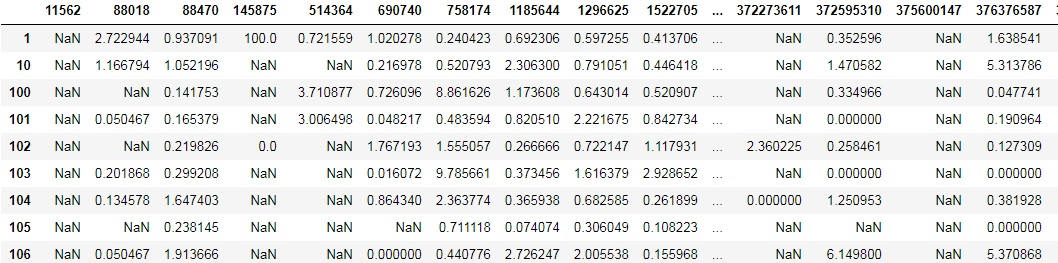
\includegraphics[scale=0.6]{./fig/matrix.jpg}
\end{center}

\noindent The similarity comparison I chose is the Pearson correlation coefficient(PCC) which measure the linear correlation of 2 people based on their interested in a set of items. In our case, the interests are the scores of 120 heroes. PCC is calculated by [2]:

\begin{center}
    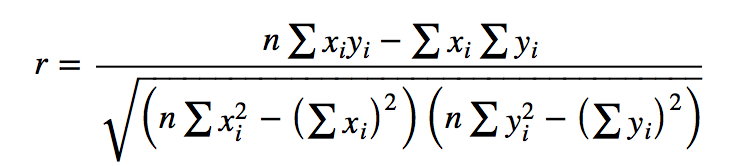
\includegraphics[scale=0.25]{./fig/PCC.png}
\end{center}

\noindent The PCC ranged from -1 to 1 which [3]:
\begin{itemize}
    \item 1: maximum positively correlated
    \item 0: non correlated
    \item -1: maximum negatively correlated
\end{itemize}

\begin{center}
    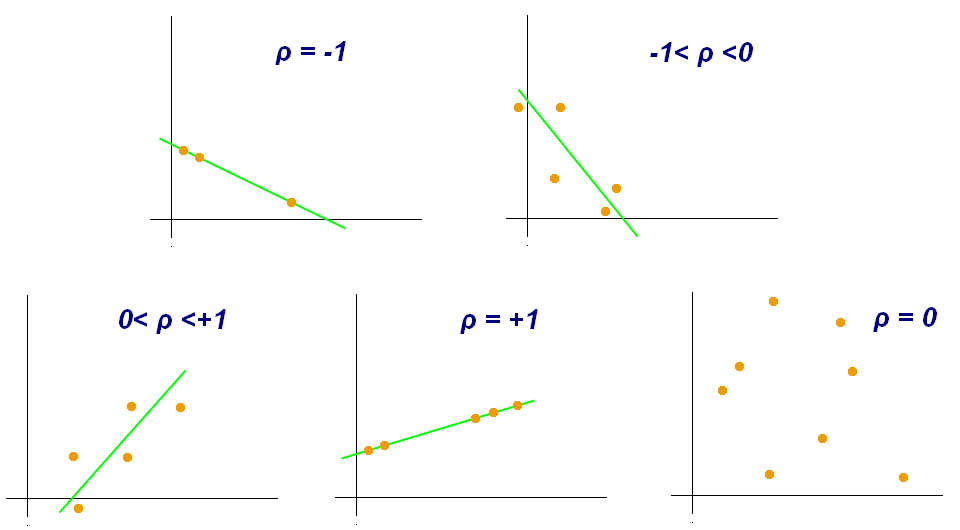
\includegraphics[scale=0.4]{./fig/Correlation_coefficient.png}
\end{center}

\noindent So we tend to recommend some heroes for the user if he has not played these heroes yet. To do that we need to predict whether he would play this hero well. Firstly, we calculated the normalized scores(same as the pro players) of the user heroes. From the dataset, we rank how similar between the user and each pro player in the dataset. The more a pro player is similar to the user, the more the user would play that hero as well as him(not so corrected since they are pros but everyone wants to be a pro then). Then, the predicted unplayed heroes score is calculated by weighting average(higher rank = higher weight) [2]. We return the highest predicted score heroes and bonus the user best-perfomed heroes as well as which pro players are most similar to him.


\section{Questions}

\subsection{Which tech stacks/frameworks (backend, database, frontend if applicable) you choose to build your APIs? You should also discuss the Pros and Cons of all the various technologies you considered}

For the backend, I choose python Flask framework and PostgreSQL for the database solution. I select Flask because I am familiar with Flask due to some previous projects and quick implementation since I have only one week to complete the project. I choose PostgreSQL because it is supported freely (but limited) by Heroku. \\

\noindent For data collecting, cleaning. I used numpy, pandas and regex. The dataset is stored as both csv(for quick prototyping) and json(for the web application). The reason I choose numpy, pandas is that they are open sourced softwares. The con is that I dont think pandas is scalable for backend implementation. I implemented my recommender backend by normal iterated loops not by using pandas framework. I believe spark would be suitable for scaling.

\subsection{How you can improve the APIs further in the long term (i.e. product roadmap that includes a brief description of why the features are useful)}

For the leaderboard API, I would suggest adding one more field, last updated date. Therefore, we can update the entries after a period (it is a tradeoff between quick response and fresh data response). Secondly, I should build a front-end for the product. All the future improvements to the code base, I already put a [TODO] mark to each section. \\

\noindent For the heroes recommender API, firstly I want to improve the calculating score function by adding some factor like weighting player recent performances. The most important thing is to have a database implementation for the recommender system, more data would result in the more accurate results. \\

\noindent Moreover, I have an idea to maintain a graph based recommender but dont have enough time to try.

\subsection{Why you choose the open API(s) that you used}

I choose the OpenDotaAPI as recommended and I don't have much time to explore any other APIs. Compared to the Dota2 API, it has more options and requests. With OpenDotaAPI, I don't need to provide the specific host which is slightly comfortable to test the web app on both localhost and server without worrying about changing the API key. \\

\noindent The con is that it is costly. Only free for 50,000 per month and after that \$0.01 per 100 requests which is a factor to concern when we consider a commercial product.

\subsection{For API \#3, why is your recommendation engine good?}

Some interesting results while I test the APIs:
\begin{itemize}
    \item S4(id=41231571) is similar to Arise(id=96169991)
    \item Loda(id=101495620) is similar to Era(id=100317750)
    \item Puppy(id=87278757) is similar to Akke(id=41288955)
    \item Sumail(id=111620041) is similar to Ferrari 430(id=88585077) and Maybe(id=106863163)
    \item w33(id=86700461) is similar to Abed(id=154715080)
\end{itemize}

\noindent For my recommendation(my id = 115202971), the system recommends me to practice Elder Titan, Tusk and Necrophos. Interestingly, I was to try playing Tusk before.

\newpage
\section{References}
\begin{enumerate}
    \item \url{https://kevintechnology.com/2013/12/30/using-machine-learning-to-recommend-heroes-for.html}
    \item \url{https://medium.com/ai-society/a-concise-recommender-systems-tutorial-fa40d5a9c0fa}
    \item \url{https://en.wikipedia.org/wiki/Pearson_correlation_coefficient}
\end{enumerate}
